\section{Experiments}
\label{sec:experiments}
In this section, we conduct experiments with the aim of
answering the following research questions:
\begin{enumerate}
\item[\textbf{RQ1}] Does our proposed \emph{GAttN with RLfD} method outperform the baseline methods in exact-K recommendation problem?
\item[\textbf{RQ2}] How does our proposed \emph{Graph Attention Networks} (GAttN) framework work for modeling the problem?
\item[\textbf{RQ3}] How does our proposed optimization framework \emph{Reinforcement Learning from Demonstrations} (RLfD) work for training the model?
\end{enumerate}
\subsection{Experimental Settings}
\subsubsection{Datasets}
We experiment with three datasets and Tab. \ref{tab:dataset_statistic} summarizes the statistics.
The first two datasets are constructed from MovieLens
and last dataset is collected from real-world exact-K recommendation system on Taobao platform.
%To construct the training and test sets, we perform a 4:1 random splitting as in \cite{wang2017irgan} for all the datasets.
The implementation details and parameter settings can be found in Appx. \ref{sec:implementation}.
%\begin{table}[h]
%	\vspace{-10pt}
%	\caption{Statistics of the experimented datasets.}
%	\vspace{-10pt}
%	\label{tab:dataset_statistic}
%	\centering
%	\scriptsize
%	\begin{tabular}{c|c|c|c|c}
%		\toprule
%		\textbf{Dataset} & \textbf{User\#} & \textbf{Card\#} & \textbf{Item\#} & \textbf{Sample\#} \\
%		\midrule
%		MovieLens(K=4,N=20) & 817 &  & 1630 & 40036 \\
%		\midrule
%		MovieLens(K=10,N=50) & 485 &  & 1649 & 33198 \\
%		\midrule
%		Taobao(K=4,N=50) & & &  & 116582 \\
%		\bottomrule
%	\end{tabular}
%	\vspace{-10pt}
%\end{table}

\paragraph{\textbf{MovieLens.}}
This movie rating dataset\footnote{\url{http://grouplens.org/datasets/movielens/100k/}} has been
widely used to evaluate collaborative filtering algorithms in RS.
As there is no public datasets to tackle exact-K recommendation problem,
we construct for it based on MovieLens.
While MovieLens is an explicit
feedback data,
%we mainly focus on the implicit feedbacks in real-world problem.
%To this end,
we first transform it into implicit
data, where we regard the 5-star ratings as positive feedback and treat all other entries as unknown feedback \cite{wang2017irgan}.
Then we construct recommended cards of each user with set of $K$ items\footnote{The $K$ items in a card are randomly permuted. As we suppose in Sec. \ref{sec:problem_definition}, the permutation of the $K$ item is not considered.},
where cards containing positive item are regarded as positive cards (labeled as 1) and cards without any positive item are negative cards (labeled as 0).
Meanwhile, positive item in the corresponding card can be seen as what user actually clicked or preferred item belonging to that card.
Finally we construct a candidate set with $N$ items for each card for a user, 
where the $N$ items are randomly sampled from the whole items set given this user and must include all the items in that card.
We show examples how the dataset like in Tab. \ref{tab:dataset_example}.
Specially in our experiments, we construct two dataset:
1) card with $K=4$ items along with $N=20$ candidate items and 
2) card with $K=10$ items along with $N=50$ candidate items.
We call the above two dataset as \textbf{MovieLens(K=4,N=20)} and \textbf{MovieLens(K=10,N=50)}.
%in the following experiments.
%The trainable embedding size for input user and item id is set as 16.
Notice that there is no constraint between items in the output card (i.e $C=\emptyset$ defined in Sec. \ref{sec:problem_definition}) for these two datasets.
%\begin{table}[h]
%\vspace{-10pt}
%\caption{Show case of the dataset. We take $K=4$ and $N=20$ for example. Items and users are represented as IDs here.}
%\vspace{-10pt}
%\label{tab:dataset_example}
%\centering
%\scriptsize
%%\begin{threeparttable}
%\begin{tabular}{c|c|c|c|c|c}
%	\toprule
%	& \textbf{user} & \textbf{card} & \textbf{candidate items} & \textbf{card label} & \textbf{positive item} \\
%	\midrule
%	sample\#1 & 1 & 1,2,3,4 & 1,2,3,4,...,20 & 1 & 2 \\
%	\midrule
%	sample\#2 & 1 & 1,4,5,6 & 1,2,3,4,...,20 & 0 & / \\
%	\bottomrule
%\end{tabular}
%%\begin{tablenotes}
%%	\footnotesize
%%	\item (We take $K=4$ and $N=20$ for example. Items and users are represented as IDs here. )
%%\end{tablenotes}
%%\end{threeparttable}
%\vspace{-10pt}
%\vspace{-10pt}
%\end{table}

\paragraph{\textbf{Taobao.}}
Above two datasets for exact-K recommendation problem based on MovieLens are what we call synthetic data which are not real-world datasets in production.
On the contrary, we collect a dataset from exact-K recommendation system in Taobao platform,
of which two days' samples are used for training and samples of the following day for testing,
and specifically with $K=4$ and $N=50$.
We call it \textbf{Taobao(K=4,N=50)}.
%\yu{The same with MovieLens. datasets.}
%The components of this dataset is the same with above MovieLens based two datasets as shown in Tab. \ref{tab:dataset_example}.
%In this dataset, the feature vectors for user and item are statistic features with size of 40 and 52, instead of ID features.
Notice there is a required constraint between items in the output card in this dataset,
that normalized edit distance (NED) \cite{marzal1993computation} of any two items' titles must be larger than $\tau=0.5$, i.e $C=\{NED(a_i,a_j)\geq\tau|a_i\in A,a_j\in A,i\neq j\}$ defined in Sec. \ref{sec:problem_definition},
to guarantee the diversity of items in a card.

\subsubsection{Evaluation Protocol}
For evaluation, we can't use traditional ranking evaluation metrics such as nDCG, MAP, etc. 
These metrics either require prediction scores for individual items or assume that ``better'' items should appear in top ranking positions,
which are not suitable for exact-K recommendation problem.
\paragraph{\textbf{Hit Ratio}} 
Hit Ratio (HR) is a recall-based metric, measuring how much the
testing ground-truth $K$ items of card $A^*$ are in the predicted card $A$ with exact $K$ items.
Specially for exact-K recommendation, we refer to HR@K and is formulated as follows:
\begin{small}
\begin{equation}
HR@K = \left.\sum_{i=1}^{n}{\frac{|A_i\cap A_i^*|}{K}}\middle/n\right.,
\end{equation}
\end{small}
where $n$ is the number of testing samples,
$|\cdot|$ represents the number of items in a set.

\paragraph{\textbf{Precision}}
Precision (P) measures whether the actually clicked (positive) item $a^*$ in ground-truth card is also included in the predicted card $A$ with exact $K$ items,
and is formulated as follows:
\begin{small}
\begin{equation}
P@K = \left.\sum_{i=1}^{n}{I(a_i^*\in A_i)}\middle/n\right.,
\end{equation}
\end{small}
where $I(\cdot)\in\{0,1\}$ is the indicator function. 

\subsubsection{Baselines}
Our baseline methods are based on Naive Node-Weight Estimation Method (in Sec. \ref{sec:nnwem}) to adapt to exact-K recommendation.
The center part is to estimate node weight which can be seen as CTR for the corresponding item.
Therefor LTR based methods are applied and we compare with the follows:
\paragraph{\textbf{Pointwise Model.}}
DeepRank model is a popular ranking method in production which applies DNNs and a pointwise ranking loss (a.k.a MLE) \cite{he2017neural}.

\paragraph{\textbf{Pairwise Model.}}
BPR \cite{rendle2009bpr} is the method optimizes MF model \cite{koren2009matrix} with a pairwise ranking loss. It is a highly competitive
baseline for item recommendation.
%or APR \cite{he2018adversarial} or IRGAN \cite{wang2017irgan}.

\paragraph{\textbf{Listwise Model.}}
GRU based listwise model (Listwise-GRU) a.k.a DLCM \cite{ai2018learning} is a SOTA model for whole-page ranking refinement.
It applies GRU \cite{chung2014empirical} to encode the candidate items with a list-wise ranking loss.
In addition, we also compare with listwise model based on Multi-head Self-attention in Sec. \ref{sec:encoder} as Listwise-MHSA.
%Another baseline is List-CVAE \cite{jiang2018beyond} which applied Conditional Variational Auto-Encoders to learn the joint probability of the listwise items.
%But it doesn't consider constraints in model so we only evaluate it on MovieLens based datasets.
%\subsubsection{Implementation and Parameter Settings}
%Here we only report implementation details for the two datasets based on MovieLens\footnote{The code and dataset will be released.}.
%For a fair comparison, all models are set with an embedding size of $16$
%and optimized using the mini-batch Adam \cite{kingma2014adam} with a batch size of $32$ and learning rate of $0.001$. All models are trained for $10$ epoch.
%All the trainable feed-forward parameter matrices are set with the same input and output dimension as $32\times32$ (including DeepRank, RNN cells in Listwise-GRU, Listwise-MHSA and ours). 
%Specifically for our GAttN model, in decoder we use LSTM \cite{hochreiter1997long} cells and set beam size as $3$, number of heads in encoder MHSA layer is $2$, and the coefficient parameter $\alpha$ in loss function is $0.5$. For reward estimator model, we set the hidden size in fully-connected layer as 128.
\subsection{Performance Comparison (RQ1)}
Tab. \ref{tab:main_result} shows the performances of P@K and HR@K for the three datasets with respect to different methods.
First, we can see that our method with the best setting (\emph{GAttN with RLfD}) achieves the best performances
on both datasets, significantly outperforming the SOTA
methods Listwise-MHSA and Listwise-GRU by a large margin
(on average over three datasets,
the relative improvements for P@K and HR@K are
\textbf{7.7\%} and \textbf{4.7\%}, respectively).
Secondly from the results, 
we can find that listwise methods (both Listwise-MHSA and Listwise-GRU)
outperform pointwise and pariwise baselines significantly.
Therefore listwise methods are more suitable for exact-K recommendation,
because they consider the context information to represent an item (node in graph) as what we have claimed in Sec. \ref{sec:encoder}.
And Listwise-MHSA performs better than Listwise-GRU,
which indicates the effectiveness of our proposed MHSA method for encoding the candidate items (graph nodes).
More detailed analysis for our method \emph{GAttN with RLfD} can be found in the following two subsections (RQ2 and RQ3).
%(RQ2 and RQ3).
\begin{table}[h]
	%\vspace{-5pt}
	\caption{Overall performances respect to different methods on three datasets, where $*$ means a statistically significant improvement for $p<0.01$.}
	%\vspace{-10pt}
	\centering
	\scriptsize
	\begin{tabular}{c|c|c|c|c|c|c}
		\toprule
		\multirow{2}{*}{Model} & \multicolumn{2}{c|}{MovieLens (K=4,N=20)} & \multicolumn{2}{c|}{MovieLens (K=10,N=50)} & \multicolumn{2}{c}{Taobao (K=4,N=50)} \\
		\cmidrule{2-7}
		 & P@4 & HR@4 & P@10 & HR@10 & P@4 & HR@4 \\
		 \cmidrule{1-7}
		 DeepRank & 0.2120 & 0.1670 & 0.0854 & 0.1320 & 0.6857 & 0.6045 \\
		 BPR &  0.3040 & 0.2050 & 0.2350 & 0.1801 & 0.7357 & 0.6582 \\
		 %List-CVAE &  &  &  &  & / & / \\
		 Listwise-GRU & 0.4142 & 0.2423 & 0.4041 & 0.2144 & 0.7645 & 0.6942 \\
		 Listwise-MHSA & 0.4272 & 0.2465 & 0.4384 & 0.2168 & 0.7789 & 0.7176 \\
		 \textbf{Ours (best)} & \textbf{0.4743} & \textbf{0.2611} & \textbf{0.4815} & \textbf{0.2245} & \textbf{0.7958} & \textbf{0.7488} \\
		 \cmidrule{1-7}
		 Impv. & 11.0\%$^*$ & 6.1\%$^*$ & 9.8\%$^*$ & 3.6\% & 2.2\% & 4.3\% \\
		\bottomrule
	\end{tabular}
	\label{tab:main_result}
	%\vspace{-10pt}
\end{table}

\subsection{Analysis for GAttN (RQ2)}
%\yu{Performance of encoder with GRU or with MHSA.}
%\yu{Visualization of GAttN figure.}
Tab. \ref{tab:main_result} shows that Listwise-MHSA performs better than Listwise-GRU
on both P@K and HR@K on all datasets.
It indicates the effectiveness to apply MHSA method for encoding the candidate items (graph nodes).
As we claimed in Sec. \ref{sec:encoder}, 
the representation for a node should consider the other nodes in graph, 
for there can exist some underlying structures in graph that nodes may influence between each other.
Here we further give a presentational case on how the self-attention works in encoder (see Fig. \ref{fig:attention}) based on Taobao dataset.
Take item ``hat'' in graph for example, items with larger attention weights to it are kinds of ``scarf'', ``glove'' and ``hat''.
It is reasonable that users focusing on ``hat'' tend to prefer ``scarf'' rather than ``umbrella''.
So to represent item ``hat'' in graph, it's helpful to attend more features of items like ``scarf''.
\begin{figure}[th]
	%\vspace{-5pt}
	\centering
	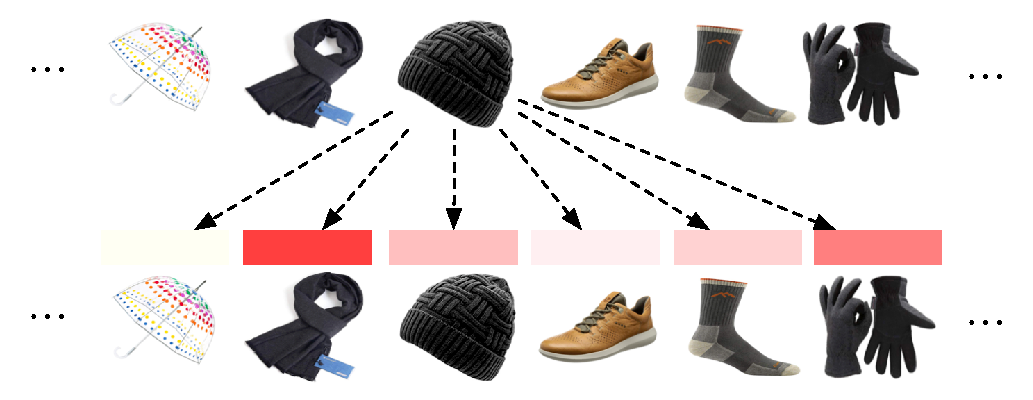
\epsfig{file=figures/attention.eps, width=0.66\columnwidth}
	%\vspace{-10pt}
	\caption{An example of the attention mechanism in the encoder self-attention in layer 2.
	The higher attention weights of the item, the darker color of the grid.
	We take item ``hat'' for example and only show attention weights in one head.}
	\label{fig:attention}
	%\vspace{-10pt}
\end{figure}

Beam search is proposed in GAttN decoder (see Sec. \ref{sec:encoder}) to expand the search space and try more combinations of items in a card to get a most optimal solution.
A critical hyper-parameter for beam search is the beam size, indicating how many solutions to search in a decoding time-step.
We tune beam size in Fig. \ref{fig:beam_search} and find that larger beam size can lead to better performances\footnote{We only report the results on MovieLens(K=4,N=20) and other datasets follow the same conclusion.} on both P@K and HR@K.
However we can also see that when beam size gets larger than 3 the improvement of performances will be minor,
so for efficiency consideration we set beam size as 3 in our experiments.
\begin{figure}[th]
	%\vspace{-10pt}
	\centering
	\epsfig{file=figures/beam_search.eps, width=0.9\columnwidth}
	%\vspace{-10pt}
	\caption{Performance of P@4 and HR@4 with different beam size in GAttN decoder.}
	\label{fig:beam_search}
	%\vspace{-15pt}
\end{figure}

\subsection{Analysis for RLfD (RQ3)}
%\yu{Supervised with or without policy-sampling, figure.}
%\yu{RL with or without hill-climbing, figure.}
%\yu{Tuned parameter $\alpha$ figure, and figure for SL v.s. SL+RL.}
To verify how our proposed optimization framework \emph{RLfD} works,
we will do the following ablation tests:
\begin{enumerate}[(1)]
\item Set $\alpha=0$ in Eq. \ref{eq:total_loss} (only reinforcement loss as Eq. \ref{eq:L_R}), and compare \emph{RL(w/ hill-climbing)} with \emph{RL(w/o hill-climbing)}.
\item Set $\alpha=1$ in Eq. \ref{eq:total_loss} (only supervised loss as Eq. \ref{eq:L_S}), and compare \emph{SL(w/ policy-sampling)} with \emph{SL(w/o policy-sampling)}.
\item Finetune $\alpha$ in Eq. \ref{eq:total_loss} and figure out the influence to the combination of SL with RL.
\end{enumerate}
Here we represent \emph{Learning from Demonstrations} and \emph{Learning from Rewards} as SL and RL for short.
Tab. \ref{tab:ablation_test} gives an overall results and we only report on dataset MovieLens(K=4,N=20) for simplification.
\begin{table}[h]
	%\vspace{-10pt}
	\caption{Performance for different settings in RLfD.}
	%\vspace{-10pt}
	\centering
	\scriptsize
	\begin{tabular}{cc|c|c}
		\toprule
		\multirow{2}{*}{} & \multirow{2}{*}{Settings in RLfD} & \multicolumn{2}{c}{MovieLens (K=4,N=20)} \\
		\cmidrule{3-4}
		& & P@4 & HR@4 \\
		\cmidrule{1-4}
		1 & RL(w/o hill-climbing) & 0.3340 & 0.2314 \\
		2 & RL(w/ hill-climbing) &  0.3573 & 0.2330 \\
		3 & SL(w/o policy-sampling) & 0.4095 & 0.2401 \\
		4 & SL(w/ policy-sampling) & 0.4272 & 0.2465 \\
		5 & RL(w/o hill-climbing) + SL(w/ policy-sampling) & 0.4495 & 0.2514 \\
		6 & RL(w/ hill-climbing) + SL(w/o policy-sampling) & 0.4472 & 0.2534 \\
		7 & \textbf{RL(w/ hill-climbing) + SL(w/ policy-sampling)} & \textbf{0.4743} & \textbf{0.2611} \\
		%RL + SL (best), $\text{reward}\in\{-1.0,1.0\}=\text{P@4}$ & 0.4450 & 0.2500 \\
		\bottomrule
	\end{tabular}
	\label{tab:ablation_test}
	%\vspace{-10pt}
\end{table}
%\begin{figure*}[th]
%	\centering
%	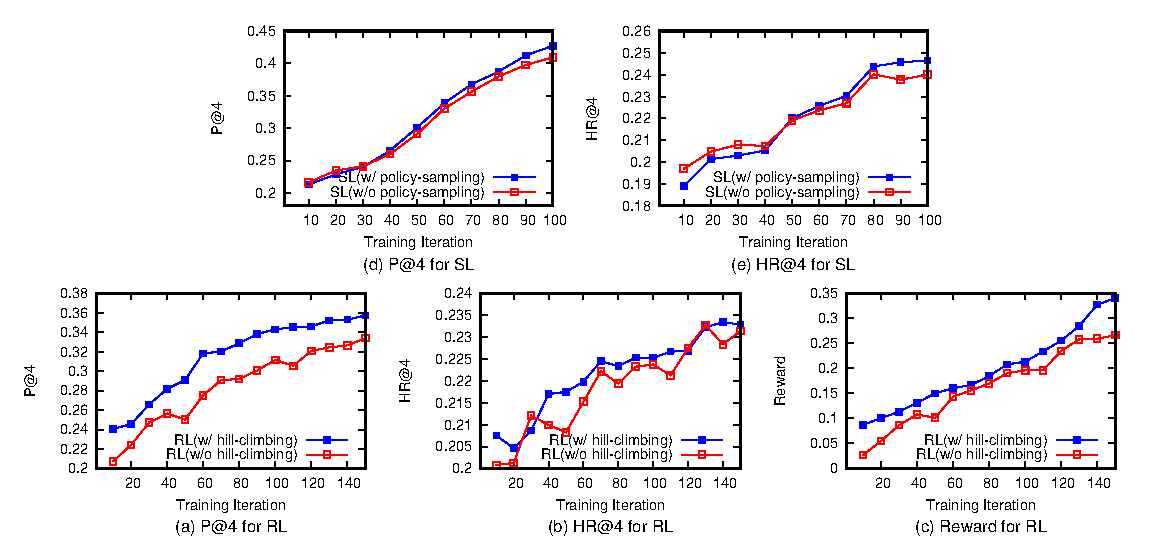
\epsfig{file=figures/curve.eps, width=1.8\columnwidth}
%	\caption{}
%	\label{fig:curve}
%\end{figure*}

Fig. \ref{fig:hill_climbing} shows the learning curves respect to Reward (defined in Eq. \ref{eq:reward}), P@4 and HR@4 for RL with (w/) or without (w/o) hill-climbing proposed in Sec. \ref{sec:reinforce}.
From the curves, we can find that with the help of hill-climbing REINFORCE training becomes more stable and steadily improves the performance, 
finally achieves a better solution (row 1 vs. 2 and row 5 vs. 7 in Tab. \ref{tab:ablation_test}).
Another insight in Fig. \ref{fig:hill_climbing} is that learning curve of Reward is synchronous monotonous with P@4 and HR@4,
which verifies the effectiveness of our defined reward function to direct the objective in problem.
\begin{figure}[th]
	%\vspace{-10pt}
	\centering
	\epsfig{file=figures/hill_climbing.eps, width=0.9\columnwidth}
	%\vspace{-10pt}
	\caption{Learning curves respect to Reward, P@4 and HR@4 for RL with (w/) or without (w/o) hill-climbing.}
	\label{fig:hill_climbing}
	%\vspace{-10pt}
	%\vspace{-5pt}
\end{figure}

Fig. \ref{fig:policy_sampling} shows the learning curves respect to P@4 and HR@4 for SL with (w/) or without (w/o) policy-sampling proposed in Sec. \ref{sec:supervise}.
We observe that in the beginning 50 iterations SL with policy-sampling may perform worse than without policy-sampling.
We believe that in the first steps of training procedure the learned policy can be poor,
so feeding the output sampled from such policy to the next time-step as input in decoder can lead to worse performances.
However as training goes on, SL with policy-sampling will converge better for revising the inconsistency between training and inference of policy,
finally achieve better performances (row 3 vs. 4 and row 6 vs. 7 in Tab. \ref{tab:ablation_test}).
\begin{figure}[th]
	%\vspace{-10pt}
	\centering
	\epsfig{file=figures/policy_sampling.eps, width=0.9\columnwidth}
	%\vspace{-10pt}
	\caption{Learning curves respect to P@4 and HR@4 for SL with (w/) or without (w/o) policy-sampling.}
	\label{fig:policy_sampling}
	%\vspace{-10pt}
	%\vspace{-5pt}
\end{figure}

In Fig. \ref{fig:coefficient} we tune hyper-parameter $\alpha$ defined in Eq. \ref{eq:total_loss},
which represents trade-off for applying SL and RL in training process.
We observe that $\alpha=0.5$ achieves the best both on P@4 and HR@4.
The performances increase when
$\alpha$ is tuned from 0 to the optimal value and then
drops down afterwards,
which indicates that properly combining SL and RL losses can result in the best solution.
Furthermore, we find that when only apply SL loss ($\alpha=1$) we can get a preliminary sub-optimal policy,
after involving some degree of RL loss the policy can be directed to achieve more optimal solutions,
which verifies the sufficiency-and-efficiency of our proposed \emph{Reinforcement Learning from Demonstrations} to train the policy.
\begin{figure}[th]
	%\vspace{-10pt}
	\centering
	\epsfig{file=figures/coefficient.eps, width=0.9\columnwidth}
	%\vspace{-10pt}
	\caption{Performance of P@4 and HR@4 with different coefficients $\alpha$ in loss defined in Eq. \ref{eq:total_loss}.}
	\label{fig:coefficient}
	%\vspace{-15pt}
\end{figure}